\documentclass[11pt,a4paper]{article}
\usepackage[utf8]{inputenc}
\usepackage{amsmath}
\usepackage{pdflscape}
\usepackage{hyperref}
\usepackage{amsfonts}
\usepackage{float}
\usepackage{graphicx}
\usepackage{amssymb}
\usepackage{parskip}
\usepackage{caption}
\captionsetup{font=footnotesize}
\title{\vspace{-2.0cm} \textbf{SENG 300: Assignment 3}}
\author{Celina Ma, John Ngo, Omar Qureshi}
\begin{document}
\maketitle
\def\textfraction{.01}
\def\topfraction{.99}

\section*{Deliverable \#1}

Of the avalible software development models, our team has chosen the scrum development model. This choice comes from the nature of our project and our client avaliability - our project is new and novel to all of us, requiring a high degree of experimentation and clarification. Furthermore, we are able to communicate with our client by email on a daily basis if need be, and a weekly basis in person as well. The project size is also considerable.

Firstly, based off these aspects of our project, most incremental models are not ideal. Incremental models are best when we can get a definite idea of what we want from our client and know what we can or cannot do. Furthermore, they tend to be based off a heavy initial requirements gathering phase with a client, followed by an implementation phase where client feedback is impossible or not needed. Concurrant and waterfall style both fall under this incremental category. However, in our project, we did not have a clear, definitive idea of what our client wants. This project is also novel and experimental, and as such we do not have a clear sense of what we can/cannot do and how to do so. Finally, we can meet with our client on a weekly basis and communicate on a daily basis - to follow an incremental model would thus squander this advantage. As such, neither incremental model has been chosen.

Opportunistic model is best on tiny projects, preferably one without a client. We have a client, and our project is not small, being more than a hundred lines of code. As such, the opportunistic model is a bad fit for our project and is not chosen.

We had considered choosing the Spiral model at first, and at first it seemed like a good fit. Spiral is ideal for long term projects with occasional periodic communication with our client. However, it also requires that we know how to do risk assessment, which we had yet to learn, and it is made of short waterfall bursts, which possess all of the downsides of waterfall within the one burst. As our project time is incredibly short as well, for the purposes of this class, it turns out that spiral is not a good fit - we did not know risk assessment, nor did we have the time to make use of the iteration desired and given by spiral.

This leaves the scrum model. In the scrum model, we gather requirements into a project backlog, and then with communicaton and client-centric feedback, we work on tackling and handling each requirement within the backlog, with changes simply being more additions to the backlog. Scrum can be applied for any length of time, short or long, and being an agile methodology it allows for significant room to experiment and adjust requirements as greater understanding of the requirements and of our capacities, and of our client's desires comes up. This seems ideal for our team, where we can communicate with our client very often and adjust as needed. Indeed, in practice scrum is how our software development progressed. We also have intentions of continuing with the project after SENG, since we are working with a real world client, and as such the flexible timescale of SCRUM as opposed to Spiral further add to its value. As such, we chose the SCRUM method.


\subsection*{1-1: Functional Requrements (FRs)}

\vskip 3mm

1. "The app must be able to receive data from the muon detector."

This app must be able to communicate with the external piece of hardware in order to meet the criteria given by the client. 

\vskip 6mm

2. "The app must be able to display a 'live' reading from the muon detector."

Along with receiving input from the detector, it then must be able to display the stream of values outputted by the detector onto the phone. 

\vskip 6mm

3. "The app must be able to average out the readings when pressing the 'Summary' button"

While a live reading is displayed, the 'Summary' button takes a snapshot of the readings average after recording is finished. 

\vskip 6mm
4. "The app must be able to record the averaged  'events per min' in a table." 

After the recording ends, the values must be stored into a table that is accessible in another part/menu of the application.

\vskip 6mm
5. "The app must be able to export out the saved data to a computer so that further data interpretation and processing can be performed."

The client has specified that the readings once in tabled format must be able to export (via .csv for example) to another computer. This would progress the learning experiences of future students who want to work with the data more comfortably once it has been collected via the phone.  

\subsection*{1-2: Non Functional Requirements (NFRs)}

1. "The app should present the readings with three significant digits."

This allows the user to experience a non cluttered UI, removing unnecessary information. This NFR would fall under the usability. 

\vskip 4mm

2. "The app should record the readings by making a smooth visual animation."

A transition animation is often desired to express user action in a clearer way. This NFR would fall under the usability category. 

\vskip 4mm

3. "The app should record the readings within 0.5s after pressing the 'Start' button."

This ensures the user doesn't have to wait an unusually large amount of time to get the reading. It also stops the user from getting frustrated and pressing the button again needlessly. This NFR would fall under the response time category. 
\vskip 4mm
4. "The app should emit a feedback sound when the user presses the ‘Start' button’" 

Giving the user direct confirmation of their action being applied is helpful and again stops user from pressing the button unnecessarily. This NFR would fall under the usability category.

\vskip 4mm
5. "The app should present a relevant UI element to let the user know if the muon detector is connected or not."

This makes sure that a precondition of using the app is met, which is having the miniUSB cable plugged into the phone and detector. This NFR would fall under the learnability/usability category.



\newpage 
\section*{Deliverable \#2}

After considering both use cases and user stories, we conclude that the user stories method is a better way to represent the systems requirements for our project. Just as with the selection of our software process model, this comes from consideration of our circumstances compared to the strengths and weaknesses of each model.

The largest, most important draw of the user stories model is that it is flexible and dynamic. Its structure, where a given user wants to do something for a given reason, is how our client expresses what he wants out of the software. It is also client fairly where we can show the story cards and they would be able to understand as opposed to a use case diagram being a bit more harder to comprehend for a non technical audience. Along with the emphasis on action and reason, user stories allow for the communication of overarching requirements goals as opposed to more nitty-gritty details, which fits with the iterative model of development we have chosen, since iterative models work towards a general end goal but don’t care about details at each stage.

The largest, most important draw of the use cases model is that done correctly, it can map out the structure of the very application needed, at least to some level. However, this backbone given and its greater emphasis on specific details compared to user stories does not lend it quite as well to an iterative mode. We need to be flexible and dynamic given our short time period so changing use case diagrams is harder than changing user stories. Like mentioned, it is also more technically designed than user stories which makes it harder to communicate to our client. As such, while a decent alternative, it just doesn’t provide nearly as many advantages as with user stories in our specific case.

Therefore, we have selected user stories to represent our system requirements.


\subsection*{2-2: User Stories}

The three core functional requirements that the user (in our case Professor Donev) needs to accomplish are as follows: connect muon detector to phone, view muon detector data and save data from muon detector to a log. As such, three corresponding story cards are created; 

\newpage


\begin{figure}[h]
  \centering
  
      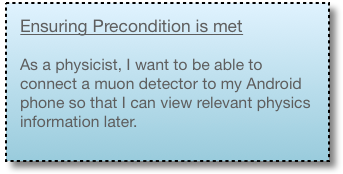
\includegraphics[width=0.7\textwidth]{storycard1.png}
  
\end{figure}

\begin{figure}[h]
  \centering
  
      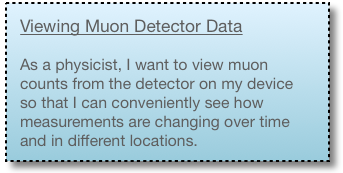
\includegraphics[width=0.7\textwidth]{storycard2.png}
     
  
\end{figure}

\begin{figure}[h]
  \centering
  
      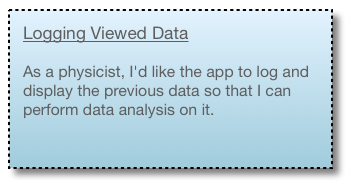
\includegraphics[width=0.7\textwidth]{storycard3.png}
      \caption{Individual story cards are first created to document core requirements, upon which further cards will be used to document how a user goes about accomplishing those tasks}
  
\end{figure}


\subsection*{2-3: Story Map}

With the use of the user story cards above, a collage/story map can be created that details further on how a user can interact with the app to accomplish their requirements. The story map can be viewed on the next landscape page;

\newpage
\begin{landscape}
\begin{figure}[h]
  \centering
  \vspace*{-2cm} \hspace*{-0.5cm}
      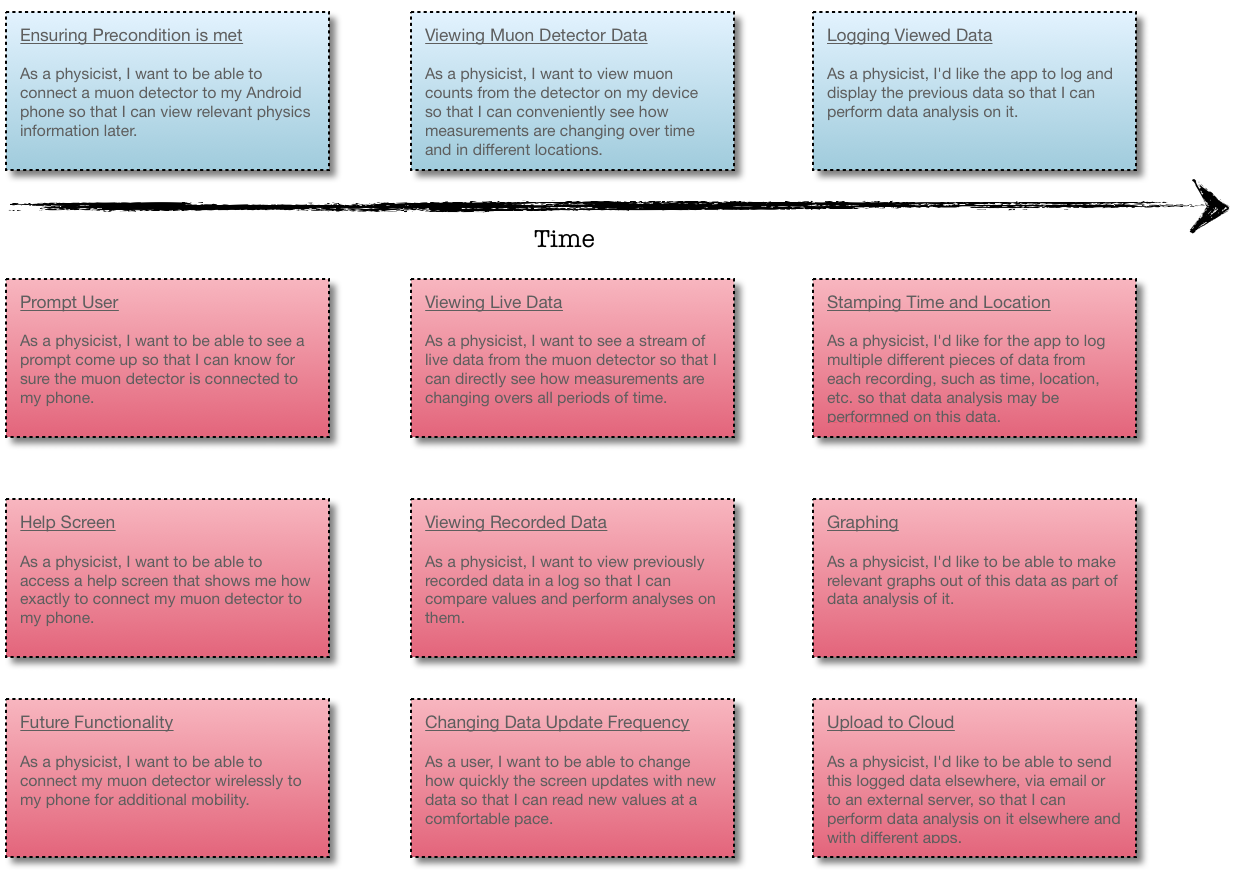
\includegraphics[width=1.9\textwidth]{storymap.png}
      \caption{A story map is used to organize requirements in order of priority and to illustrate how user interacts with app}
  
\end{figure}
\end{landscape}

\section*{Deliverable \#3}

\subsection*{3-1: Overview Sketches}
\bigskip
\begin{figure}[h]
  \centering
      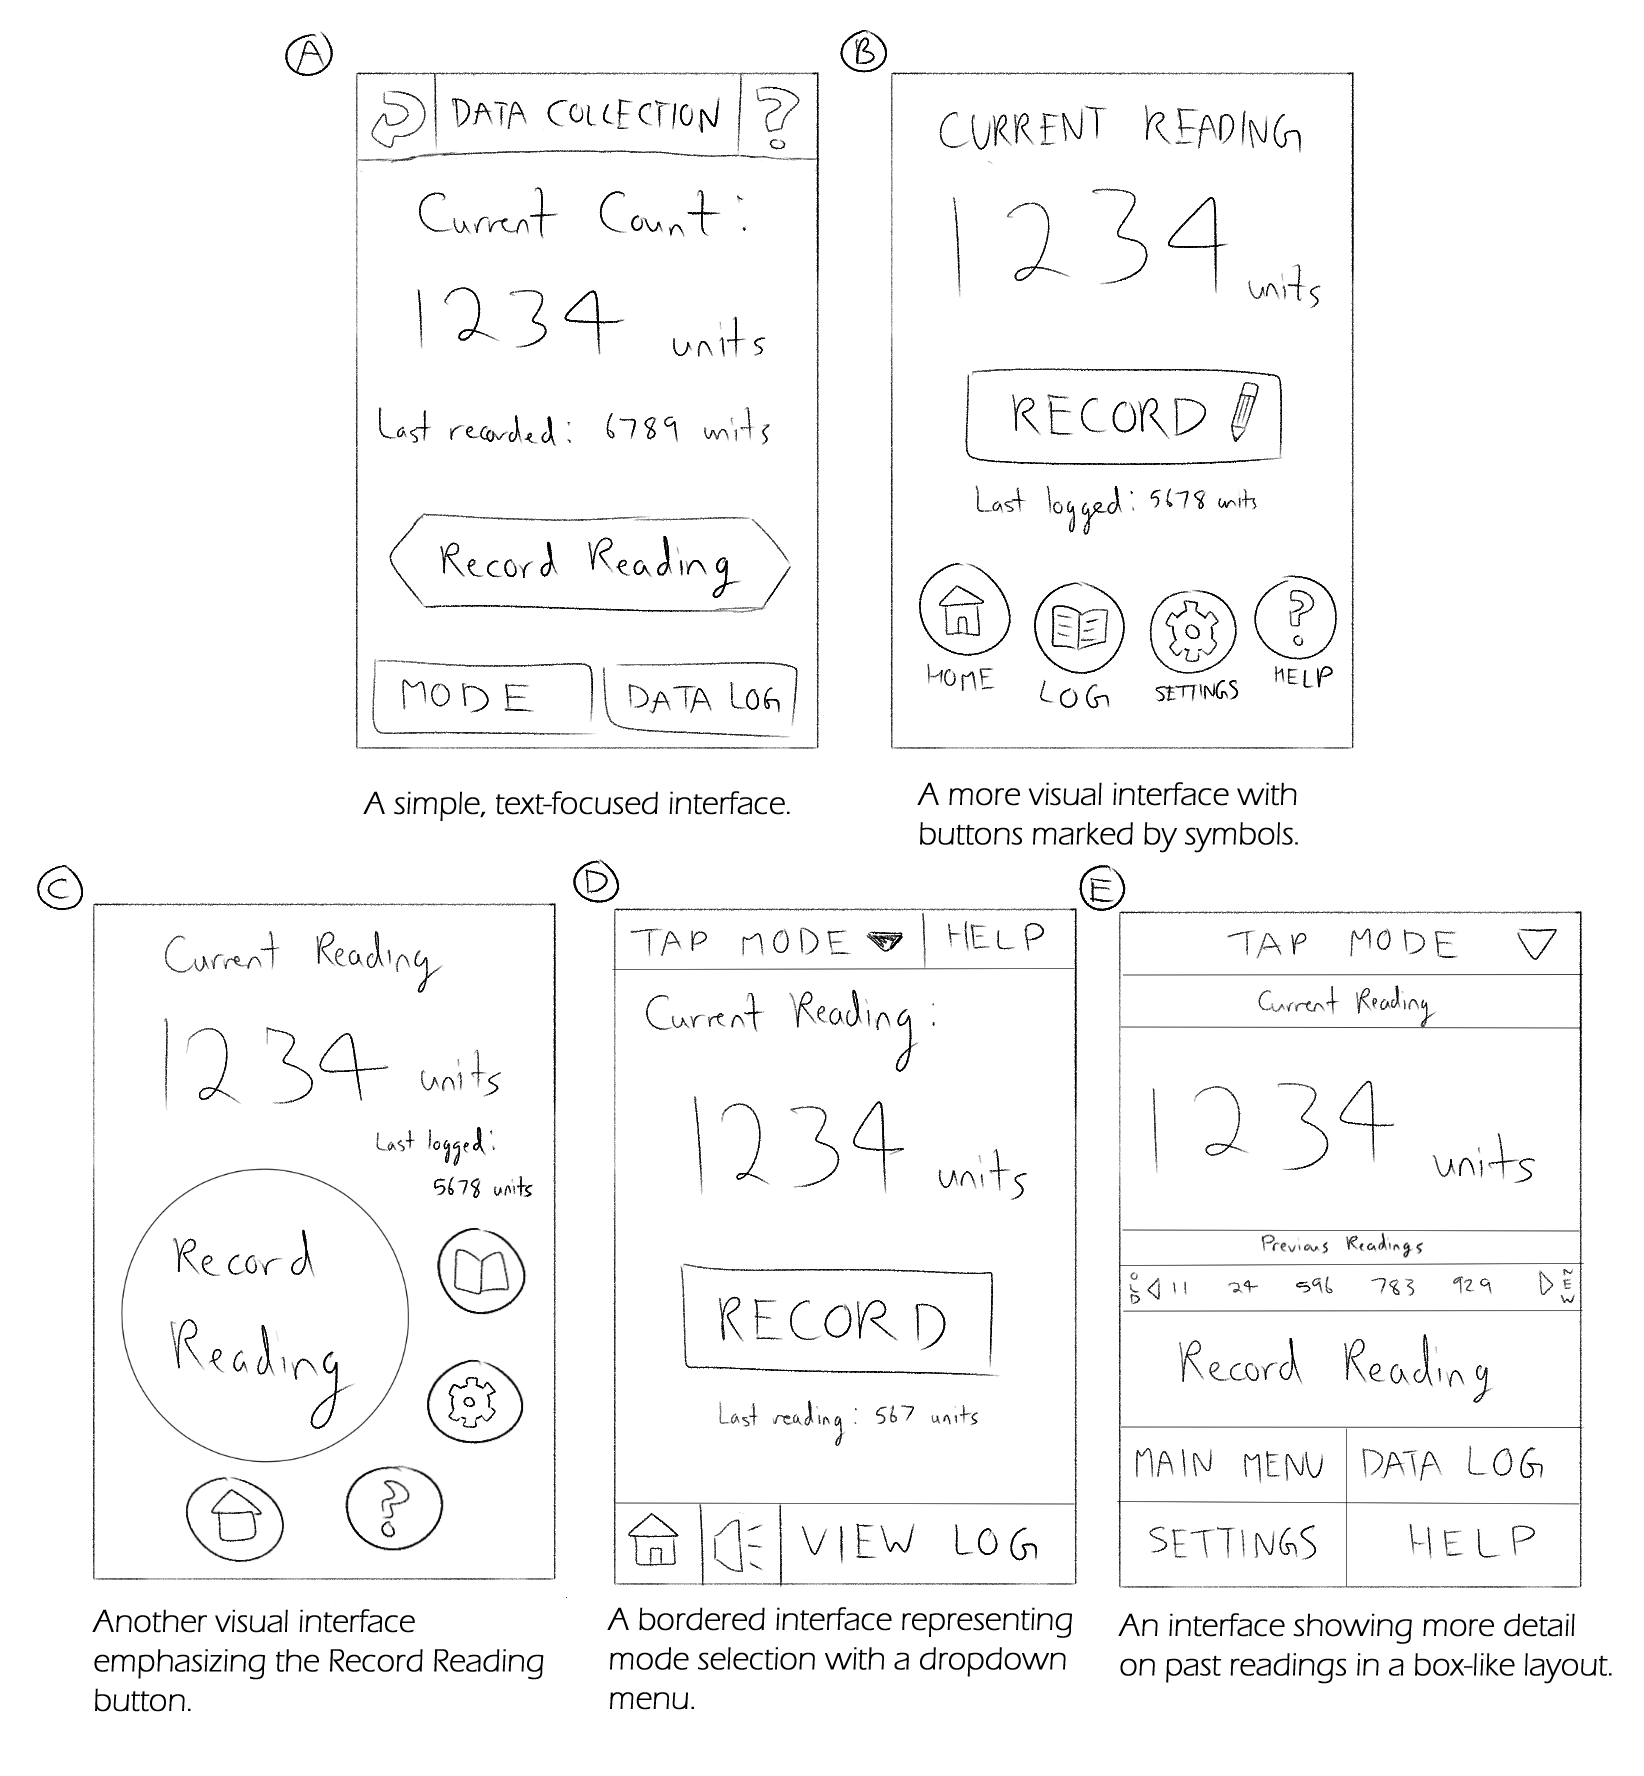
\includegraphics[width=1.1\textwidth]{overviewsketches.png}
  \caption{A variety of design approaches for the recording screen}
\end{figure}

\newpage
\subsubsection*{Why We Chose Sketch A}

We chose sketch A to elaborate on due to its clarity and emphasis on the most important aspects of this screen. The main buttons the user would interact with (Record, Mode and Data Log) are large and displayed clearly. Compared to sketches B and C, which have smaller icons that the user may accidentally mis-press, the interface of A is more focused on what is important to the user. This is key to enhancing the intuitiveness of the app. Sketch D emphasizes similar points to sketch A, but the mode selection button is somewhat less obvious in this design. Although sketch E shows more information about Previous Readings than the other sketches, it is too cluttered; additionally, that information is repeated in the Data Log screen in more detail, so it is not needed for the Data Collection screen. Thus, our main reason for choosing sketch A was its relative simplicity and correctly emphasized functions compared to the other designs.

\subsection*{3-2: Elaborating Sketches}
\def\textfraction{.01}
\def\topfraction{.99}
\bigskip
\begin{figure}[b!]
  \centering
  \hspace*{-1cm}
  \renewcommand{\textfraction}{0.05} 
      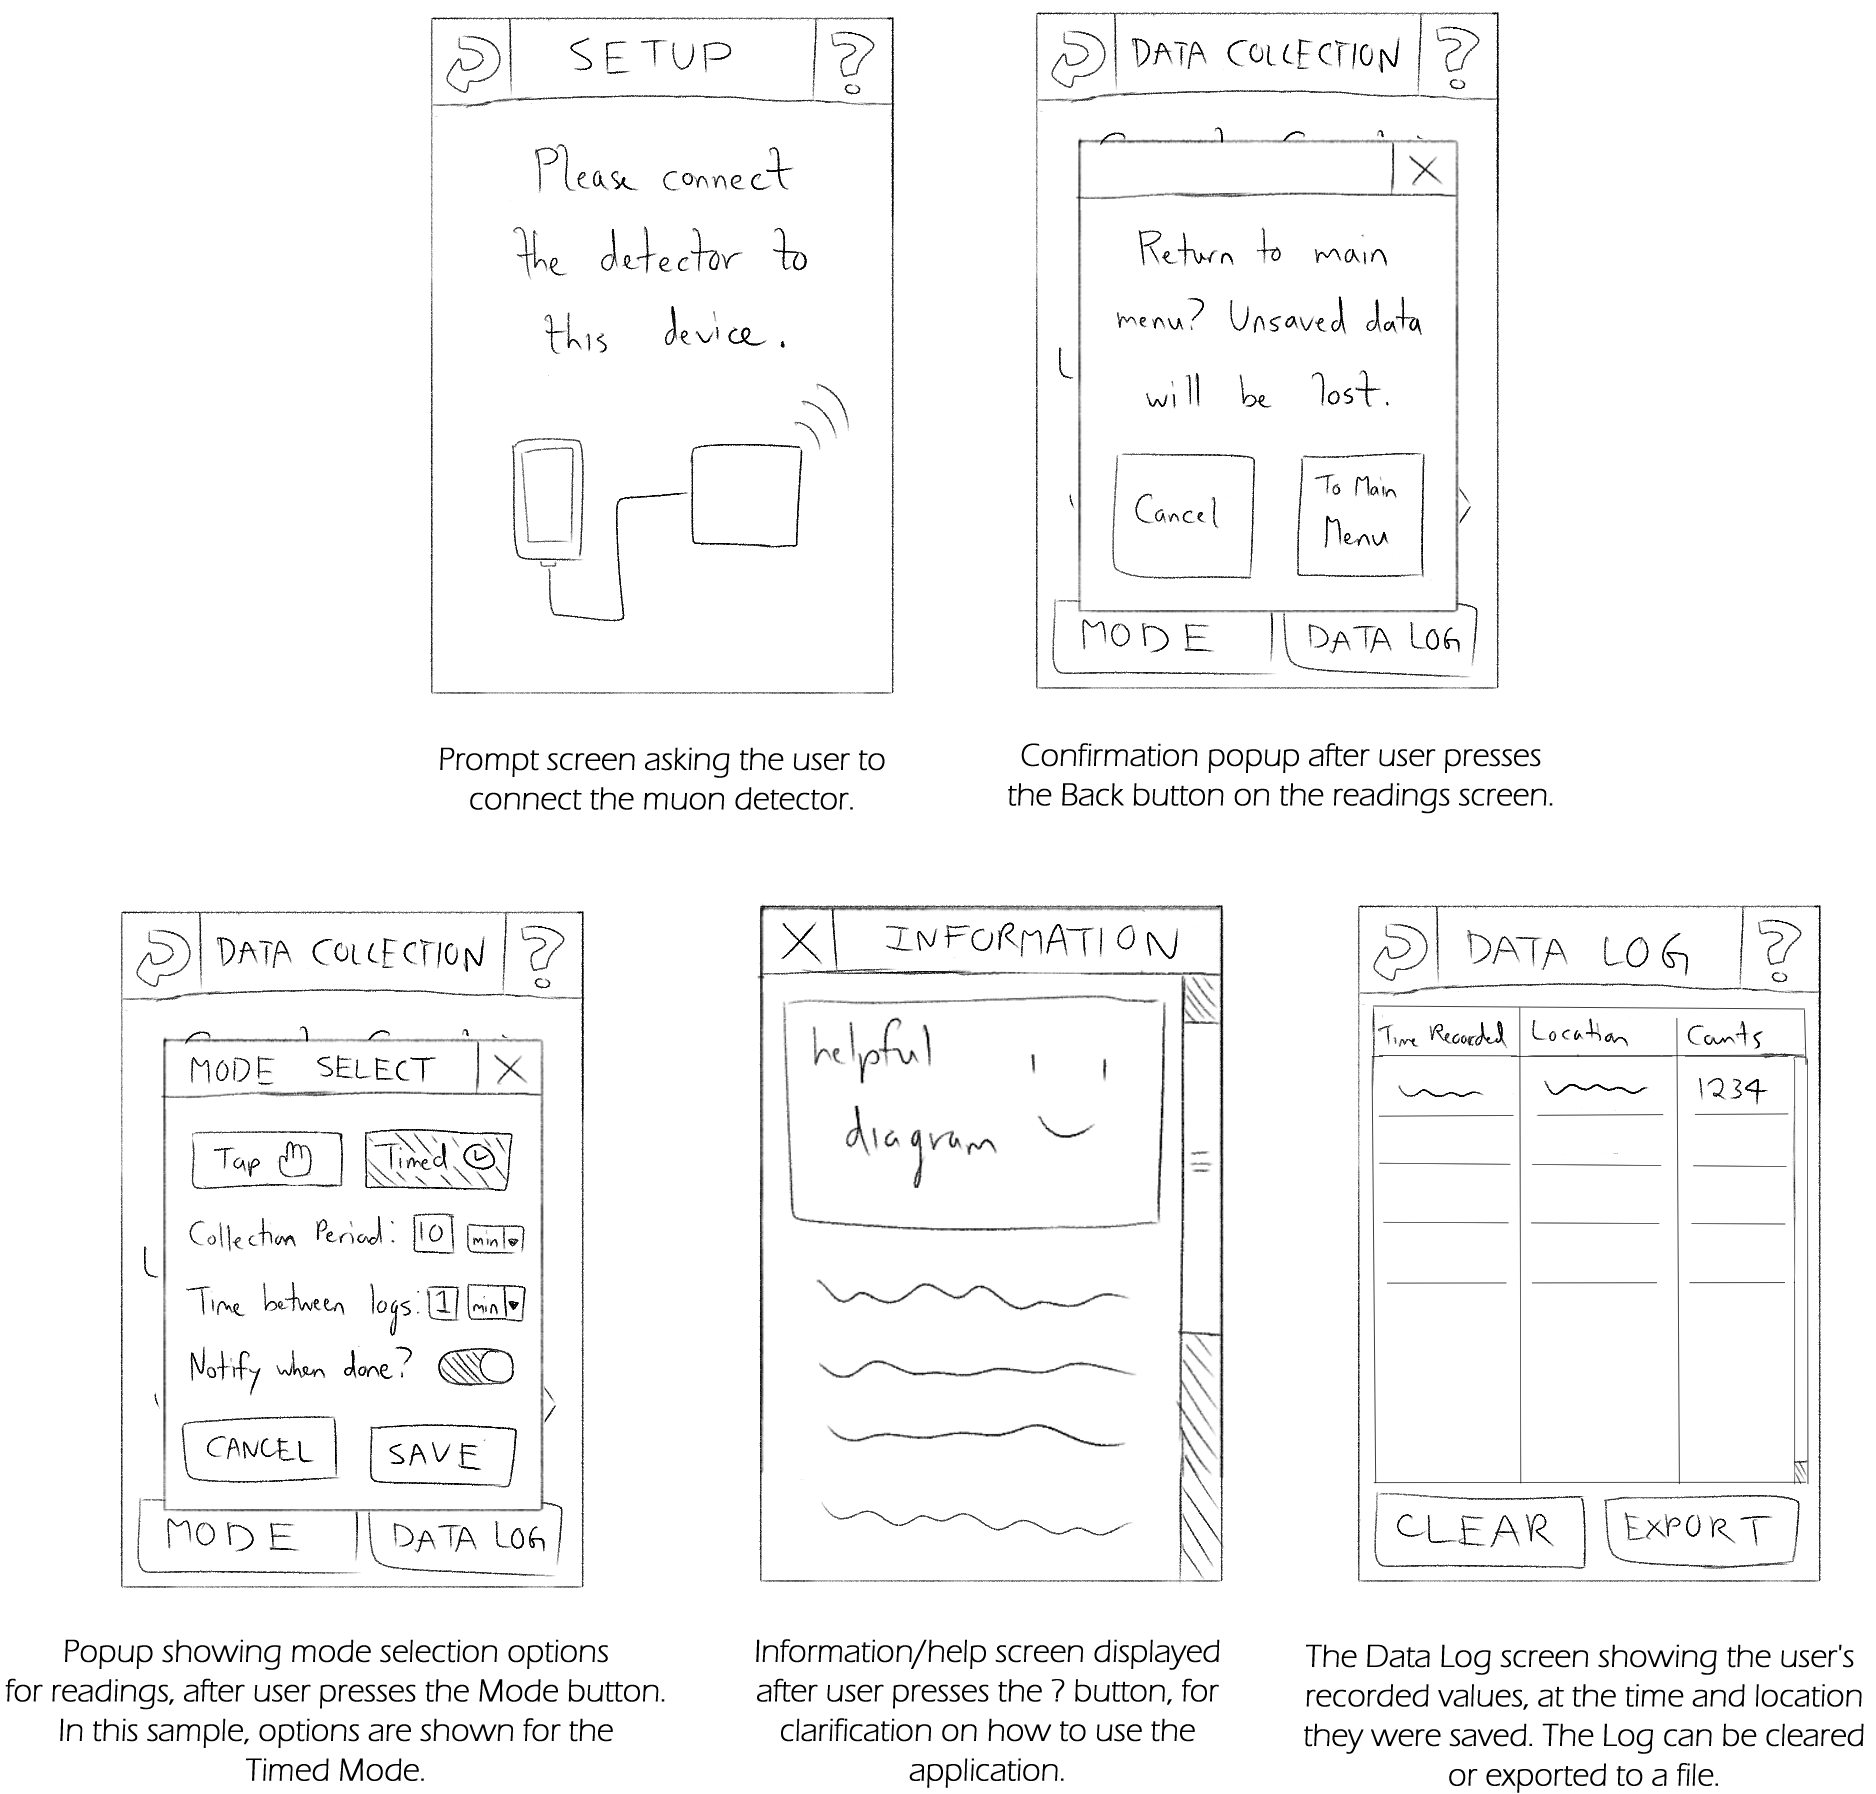
\includegraphics[width=0.84\textwidth]{elaboratingsketches.png}
  \caption{Extended sketches for other parts of the apps UI screens}
\end{figure}

\newpage
\subsection*{3-3: Storyboard Sketches}

\bigskip
\begin{figure}[h]
  \centering
  \hspace*{-0.5cm}
      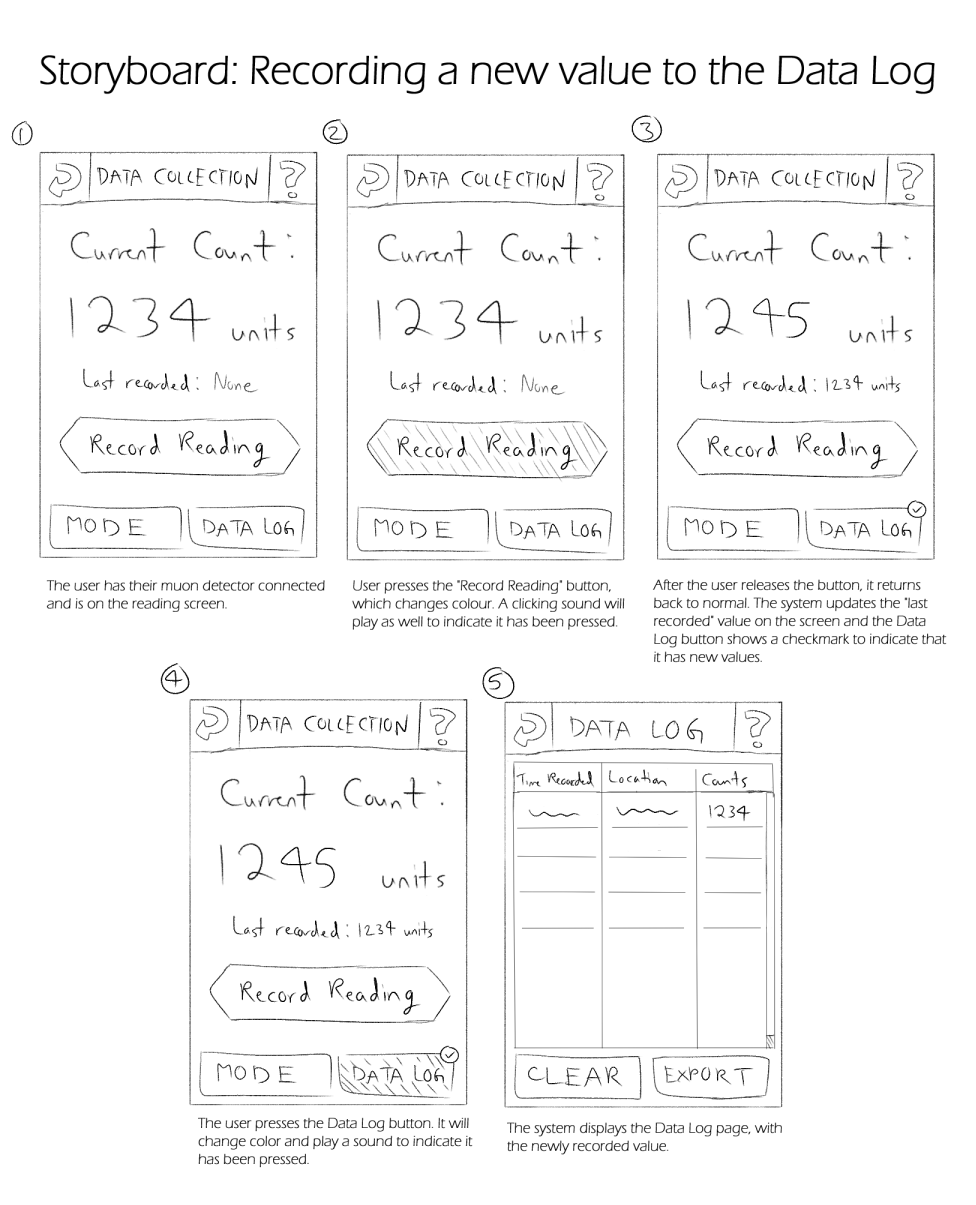
\includegraphics[width=1.15\textwidth]{storyboard.png}
  \caption{The recording screen responding to user input}
\end{figure}

\newpage
\subsection*{3-4: Wizard of Oz Demo Video}

Demo videos can be viewed below:

1. Full Video 30min (\href{https://drive.google.com/file/d/1D5OwAUCmAK5fYUDqaYs4WdFURqq9lxwS/view}{\underline{link}})

2. Short Video 1min (\href{https://drive.google.com/file/d/1GZPQ2MqETNLw6sNSMTrlxhX4ftYG58Hb/view?usp=sharing}{\underline{link}})






\section*{Deliverable \#4}
\subsection*{4-1: Poker Effort Estimation}

\begin{figure}[h]
  \centering
      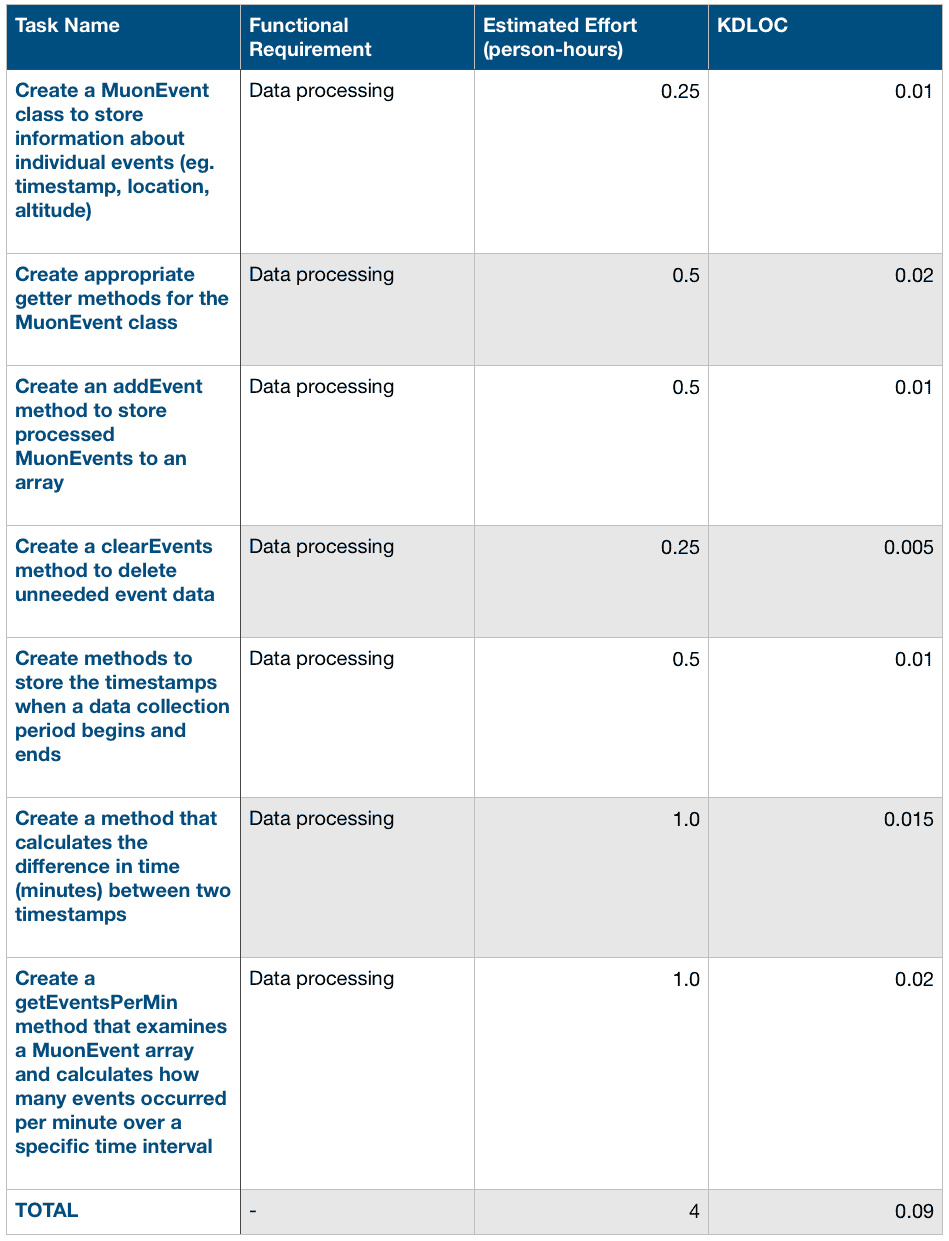
\includegraphics[width=0.8\textwidth]{dataproctable2.png}  
      \caption{Tabulating the data processing functional requirement into a set of tasks and rating them in person-hours/KDLOC}
\end{figure}

\newpage

For our planning poker session, we chose to create tasks for the following functional requirement:

\textbf{The app must process event data from the muon detector to determine the number of events per minute over a specific time interval.}

We generated seven tasks for this functional requirement and individually gave our estimates in person-hours. During our planning session, we generally had consensus for estimates, though there was some variance between us. 

For example, the task, “Create an addEvent method to store processed MuonEvents to an array”, was considered to be relatively easy by all of us. However, one person estimated the effort slightly higher and suggested that this method may need to check if the event data is valid (eg. if the timestamps are in an order that makes sense). We discussed some other issues that may occur, such as what should happen if a maximum number of events had been reached. These additional factors helped refine our estimations for person-hours of the task.

The task “calculating the difference in minutes between two timestamps” was more divisive. One of our group members believed the task would be quite difficult, requiring 5 person-hours. Another believed it would be easy requiring only 1 person-hours since Java likely contained some built-in functionality to find thet time interval difference between two date stamps. We learned that this was indeed the case and adjusted our estimations accordingly, agreeing it shouldn't take too long (1 person-hour).

We all agreed that the task of “calculating events per minute over a specific time interval” would require the most person-hours (4.0). During our discussion, we contemplated how the number of events per minute could be displayed “live” on our app screen while collecting data, since that would involve frequently saving new timestamps for the calculation. We also wondered if events per minute should only be calculated over some fixed time interval (eg. the last 10 seconds of recording) or use the whole time spent recording.

The planning poker session was useful for evaluating our list of tasks by raising new questions on generating ideas for test cases and structure. Overall, this exercise helped create estimates on the challenges to be faced when completing the functionality of the application. This also helped plan our schedules since we now had a general idea of time required for each step. 

\subsection*{4-2: Actual Effort Comparison}

Our actual efforts ended up lying close to our predicted values in person-hours for our functional requirements. To reiterate, the core functional requirements we focused on were:

\begin{enumerate}
  \item The app must be able to connect with the muon detector.
  \item The app must be able to process event data from the muon detector.
  \item The app must be able to display processed information to the user.
\end{enumerate}

The first functional requirement proved to be slightly more difficult than initially thought. Communication with the arduino based muon detector meant trying to search the internet for open source libraries such as UART or serial. The time spent searching and learning about the libraries outweighed the time actually implementing it in Java. We predicted 19 person-hours total for accomplishing all tasks of the first functional requirements but in actuality it was close to 25 person-hours.

For our second functional requirement, our predictions were pretty accurate. The two most challenging tasks of that requirement were "calculating difference between two time stamps" and "calculating events per minute over a specific time interval". Since Java functionality existed for calculating time difference between date stamps, it was simply trying to learn how to use it which took time rather the implementation. We did predict the events per minute calculation would be trickier but overall, it still lied close to our estimates. We ended up spending close to 6 person-hours on the functional requirement which was the same as the predicted value.

The last functional requirement ended up being easier than expected. We initially thought it may be time consuming configuring Android studio and working with the GUI interfaces. It was actually fairly straight forward and implementing a few screens with buttons took less time than thought. We predicted 5 person-hours for accomplishing this functional requirement when in actuality it was closer to 3 person-hours. 

In summary, the predicated values as a whole for all three functional requirements and their individual tasks lie fairly close to our estimates. In the end, it's always better to overestimate the time required to accomplish your tasks so that you can plan out your schedule and time accordingly.






\newpage
\section*{Deliverable \#5}

\subsection*{5-1: Initial Tests}

For the data processing requirement, we will focus on testing the Processor class. This class will store event data as MuonEvents occurring over some time period. Here, we see seven initial test cases that focus on checking if the correct number of events have been stored (by the getEventCount() method) and on calculating the number of events per minute. None of the test code is complete save for the expected values:

\begin{figure}[h]
      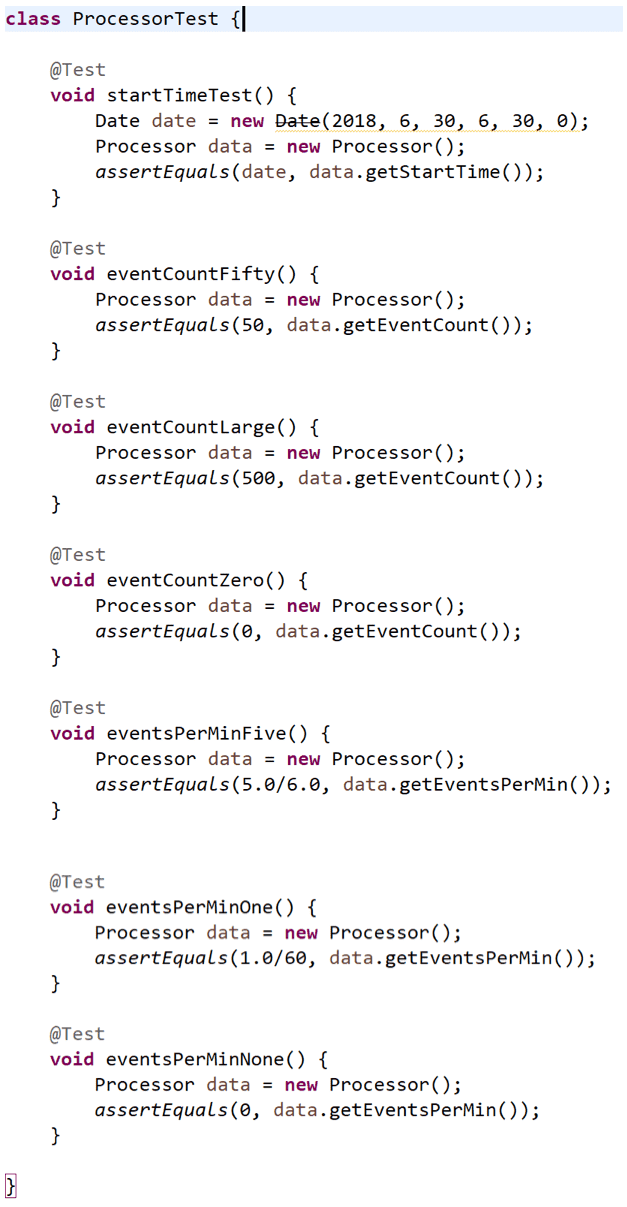
\includegraphics[width=0.63\textwidth]{codeimg1.png}  
\end{figure}

To compile the test code, a basic skeleton of the Processor class was created:

\begin{figure}[h]
	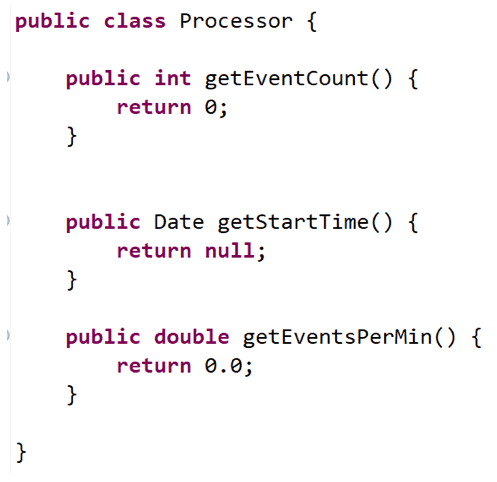
\includegraphics[width=0.63\textwidth]{codeimg2.png}
\end{figure}

When the previously created test class was now run, all but two of the tests failed. The only tests that passed already expected "0" as a result:

\begin{figure}[h]
	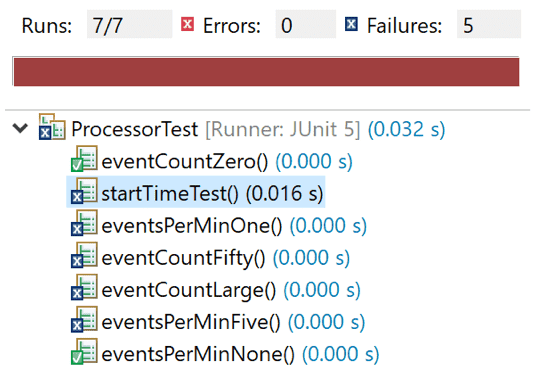
\includegraphics[width=0.83\textwidth]{codeimg3.png}
	\end{figure}
	
\newpage
\subsection*{5-2: Tests with Partial Implementation}

While working on the implementation, we realized that we needed more data and methods to flesh out the Processor class, resulting in an increased number of test cases. For example, to calculate events per minute, we needed to save the timestamps when data collection began and ended to know the length of time spent recording data. This functionality is performed by the new switchRecording method.
 
Although the full implementation of this requirement will use real muon event data from a connected muon detector, the test cases created fake data to simulate how real events would be saved by the Processor.

The following screenshots show some of the test cases after implementation:



\begin{figure}[h]
	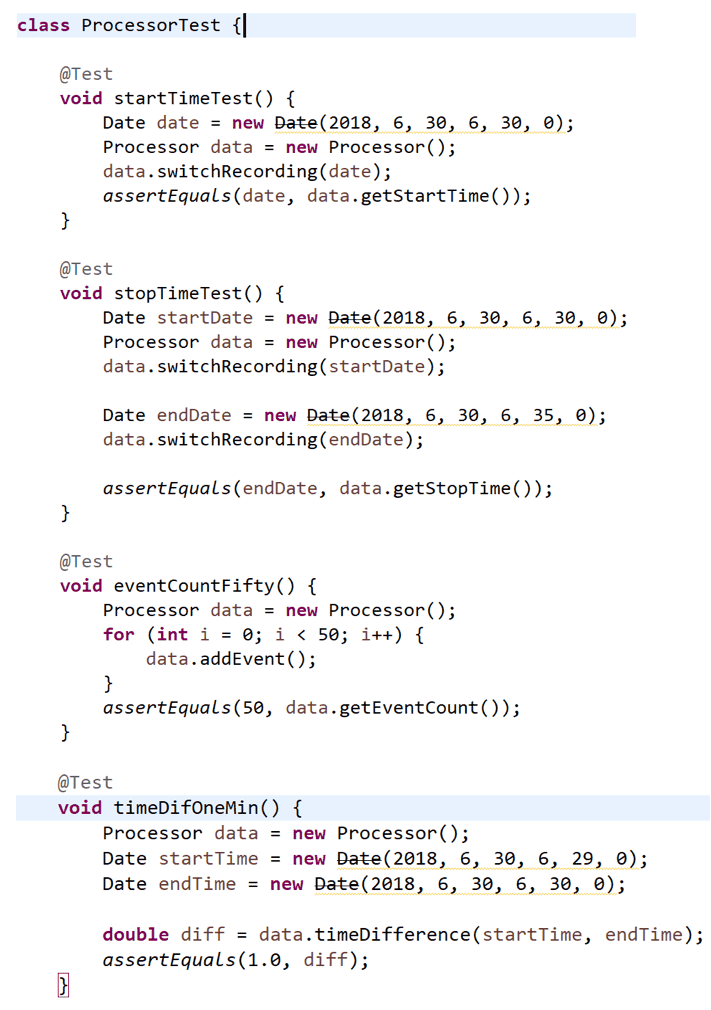
\includegraphics[width=0.79\textwidth]{codeimg4.png}
	\end{figure}

The new timeDifference method was created to calculate the difference between two timestamps in minutes. This is used in conjunction with the getEventsPerMin method:

\begin{figure}[h]
	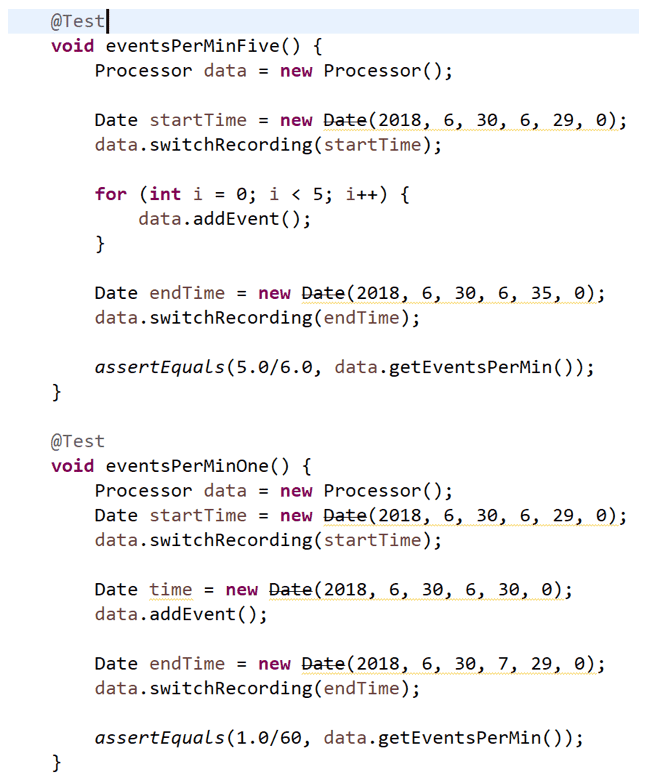
\includegraphics[width=1.0\textwidth]{codeimg5.png}
	\end{figure}
	
	
\newpage
The Processor class now has partially complete methods. However, it does not yet store instances of each muon event:

\begin{figure}[h]
	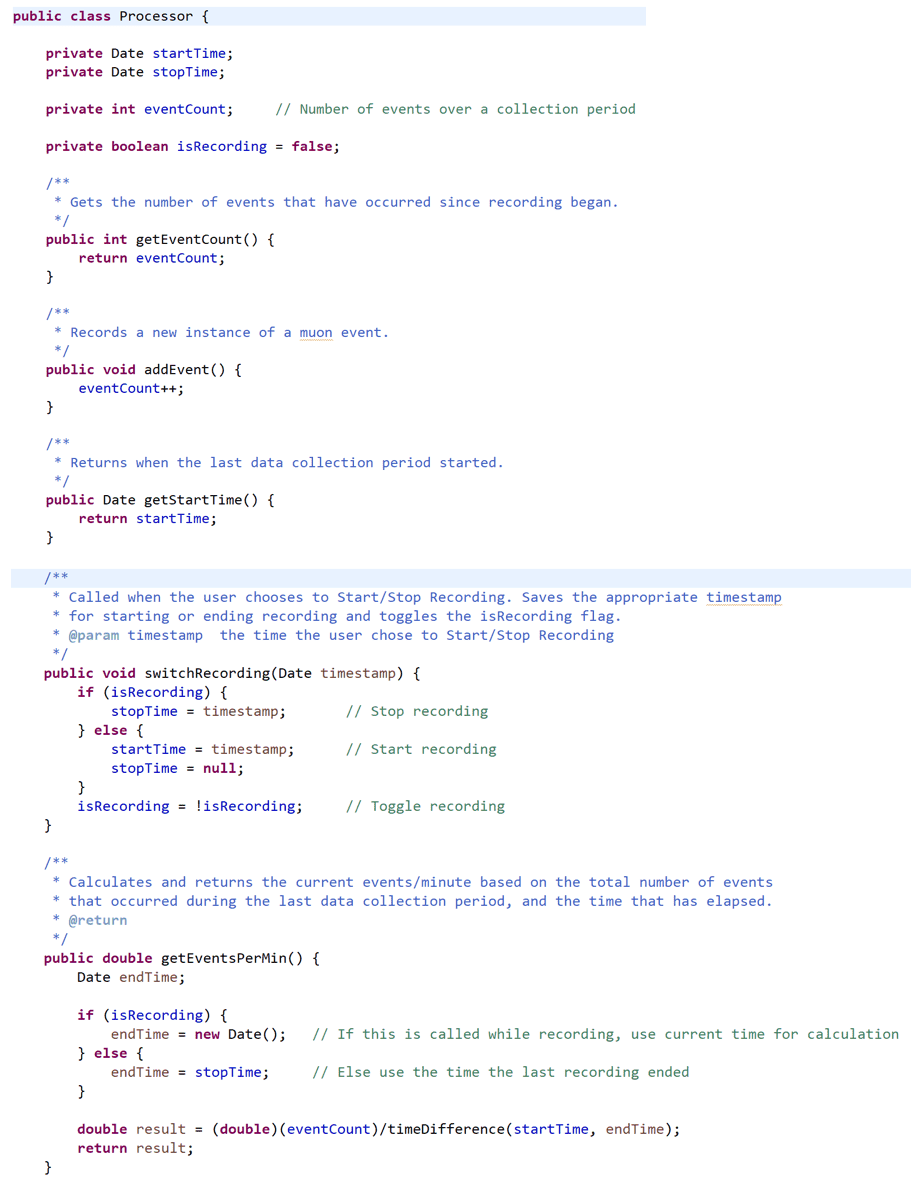
\includegraphics[width=1.1\textwidth]{codeimg6.png}
\end{figure}

\newpage

Now there is enough code to pass all the test cases:

\begin{figure}[h]
	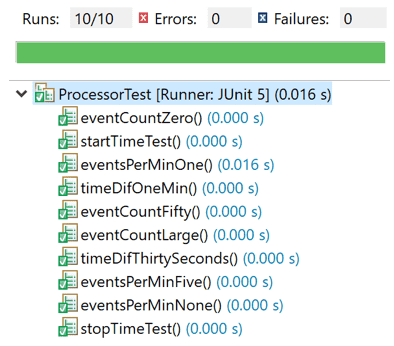
\includegraphics[width=0.7\textwidth]{codeimg7.png}
\end{figure}


\subsection*{5-3: Tests with Full Implementation}

Our demo video demonstrating the TDD approach with full implementation along with explanations can be viewed at the following (\href{https://www.youtube.com/watch?v=h2C-4-hQrhM&feature=youtu.be}{\underline{link}}).

\subsection*{5-4: Two Extra Functional Requirements}

Our demo video featuring all three functional requirements can be viewed at the following (\href{https://www.dropbox.com/s/vnuvuzx5zrtkvaa/Demo.mp4?dl=0}{\underline{link}}).



\newpage


\section*{Deliverable \#6}

\subsection*{6-1: Class Diagram}

\begin{figure}[h] \centering \hspace*{-3cm} \vspace{3cm}
	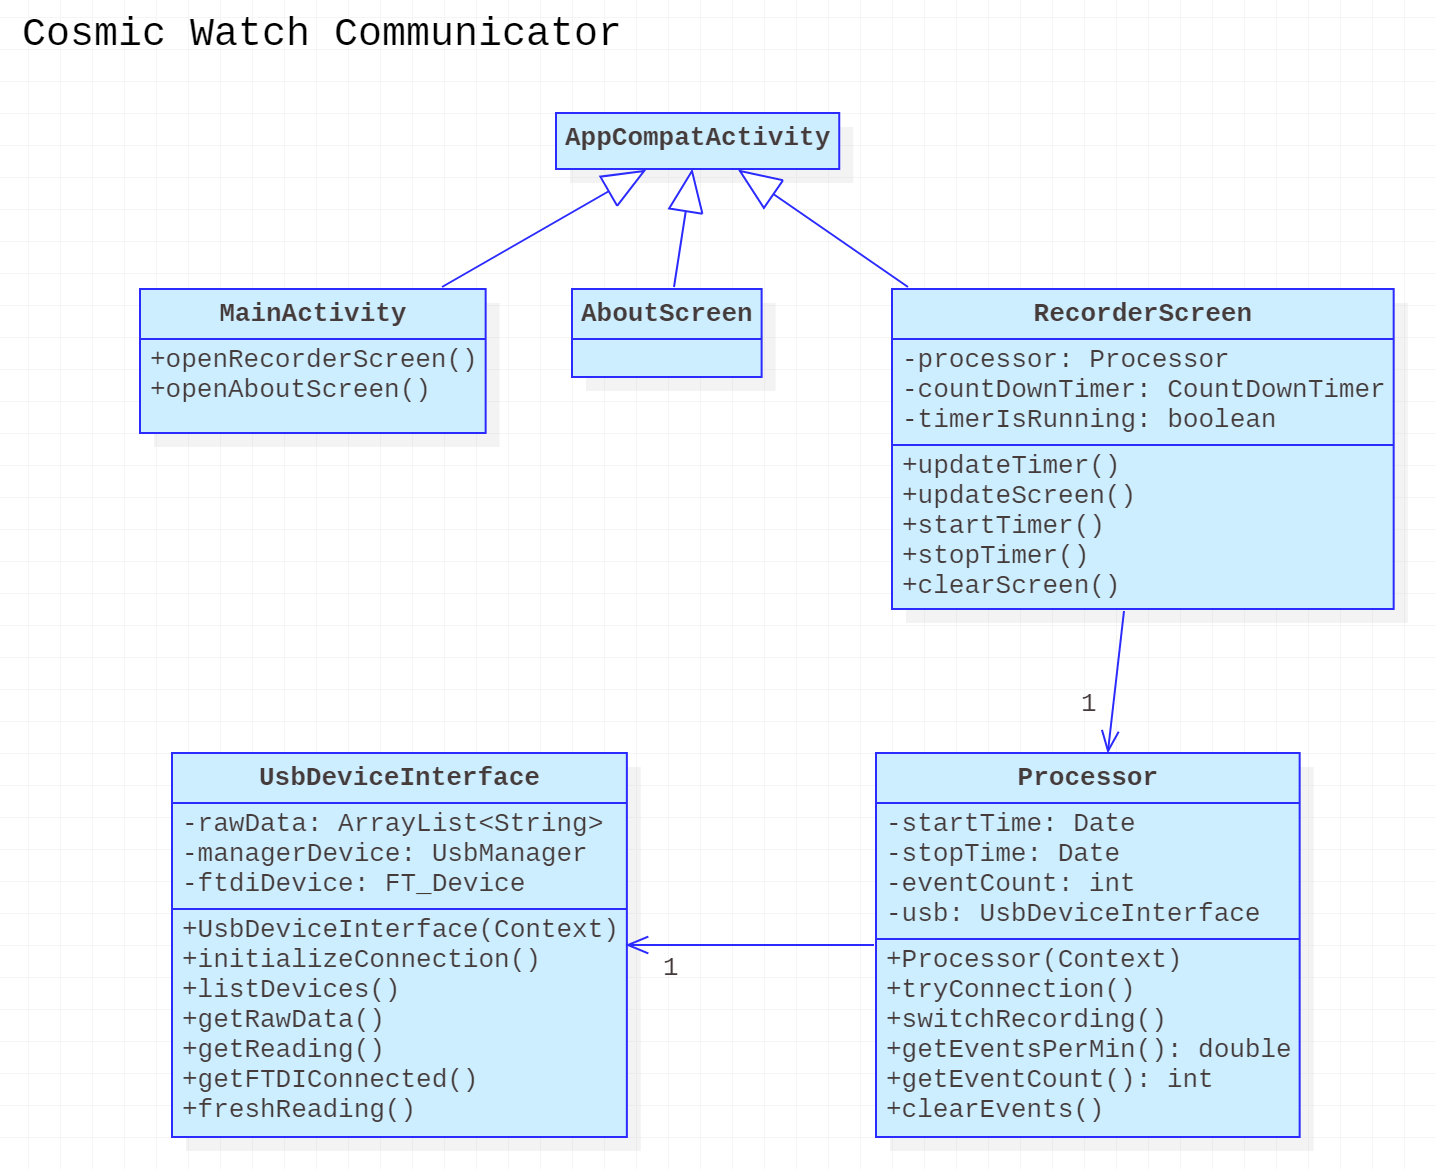
\includegraphics[width=1.5\textwidth]{classes.png}
\end{figure}
\newpage
\subsection*{6-2: Detailed Explanation}

At the top of our diagram, there are three classes extending the class AppCompatActivity. This indicates that these are the main Activities of our app, representing the screens the user can access; MainActivity, AboutScreen and RecorderScreen correspond to the Main Menu, About, and Recorder screens respectively.

The Main Menu screen allows the user to access the About and Recorder screens. Thus, MainActivity has the methods openRecorderScreen and openAboutScreen. The About screen simply displays information and has no attributes. Its only methods are onCreate and finish(), which are default Android Studio methods allowing the About screen to be displayed and closed.
RecorderScreen maintains a reference to a Processor object, which communicates between the UsbDeviceInterface and the RecorderScreen.

The RecorderScreen starts a timer when the user chooses to start recording. This is conveyed to the Processor, which will save the time recording starts and initialize the UsbDeviceInterface. The UsbDeviceInterface will open a wired connection to the muon detector and store raw data from it. When this data needs to be interpreted and displayed on the RecorderScreen, the Processor will make requests to the UsbDeviceInterface and update eventCount according to the amount of raw data saved.

When the recording session timer ends or when the user wishes to clear their saved data, the RecorderScreen sends another signal to Processor. The Processor will then reset its saved data and the raw data in UsbDeviceInterface as needed.



\newpage

\section*{Deliverable \#7}

\subsection*{7-1: Sequence Diagram 1 with Explanation}

\begin{figure}[h] \centering
	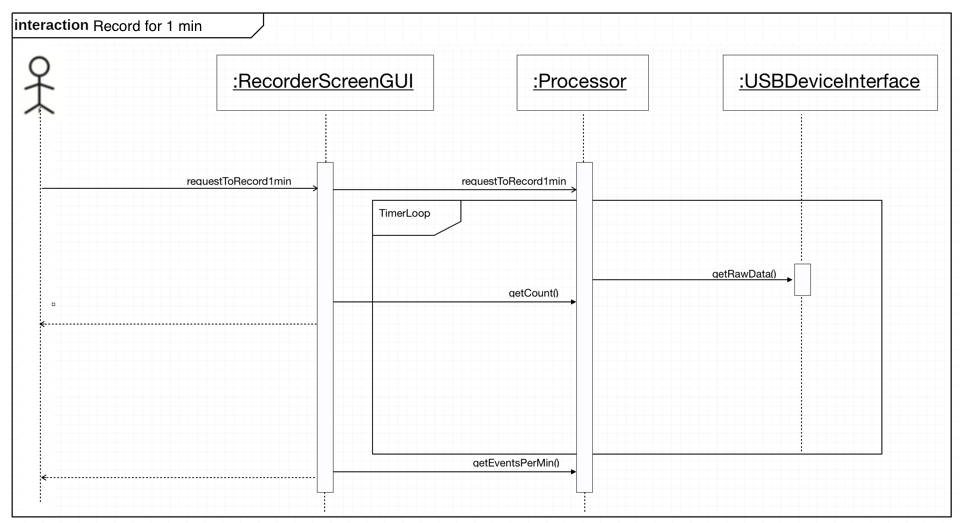
\includegraphics[width=1.08\textwidth]{sequence1.png}
\end{figure}

Our first sequence diagram demonstrates the sequence of tasks where a user initiates a recording for 1 minute. This is done by the user first being able to interact with a RecorderScreenGUI interface, specifically a button. The button communicates with the Processor class which creates a corresponding time stamp for the start of the recording session and enters into a TimerLoop for 60 seconds. During those 60 seconds, the Processor communicates with the USBDeviceInterface, which is a class used to communicate with an external piece of hardware known as a muon detector. 

As the muon detector picks up events, the Processor class calls getRawData() method from the USBDeviceInterface class increment events, which increases the private variable count in the Processor class. This happens every time a muon event occurs during those 60 seconds. The RecorderScreenGUI class then updates the count displayed by calling teh getCount() method from Processor. At the end of the TimerLoop, the RecorderScreenGUI calls the getEventsPerMin() method of the Processor class which calculates the total events that occurred divided by the total duration the recording took place by using the date stamp time difference. 

All of this information is then finally presented to the user in the RecorderScreenGUI. This entire sequence of tasks demonstrates a key concept in software engineering/computer science which is a layer of abstraction with all of the subsystems working behind the scenes while the user only interacts with a friendly UI. 

\newpage
\subsection*{7-2: Sequence Diagram 2 with Explanation}

\begin{figure}[h] \hspace{-2cm}
	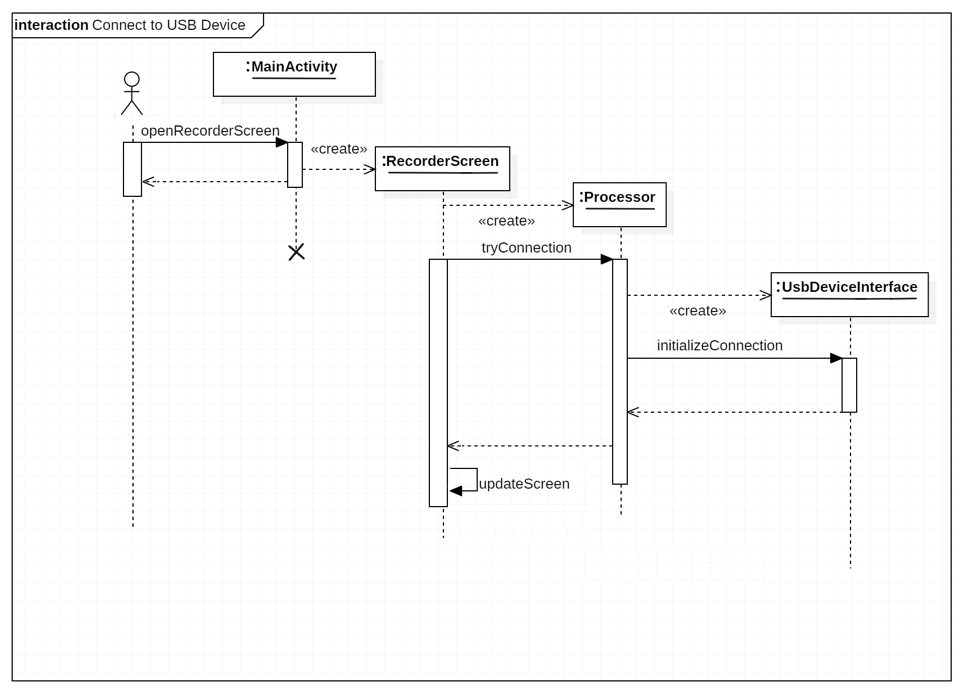
\includegraphics[width=1.3\textwidth]{sequence2.png}
\end{figure}


This sequence diagram shows the use case of the user successfully connecting to the muon detector through a USB port. When the user is on the Main Menu screen (MainActivity), they will choose to open the Recorder screen. This results in an instance of RecorderScreen being created, which also creates a Processor. MainActivity is no longer needed. 

Upon creation, RecorderScreen will ask the Processor to try to connect to the detector using the UsbDeviceInterface. The Processor will initialize the UsbDeviceInterface, and the UsbDeviceInterface will form the connection with the muon detector. After this connection is formed successfully, initializeConnection and tryConnection will return to the RecorderScreen. Finally, the RecorderScreen will display a message using updateScreen to show that the device is connected.



\newpage
\section*{Deliverable \#8}

\subsection*{8-1: Class Diagram with Design Pattern}

\begin{figure}[h] \centering
	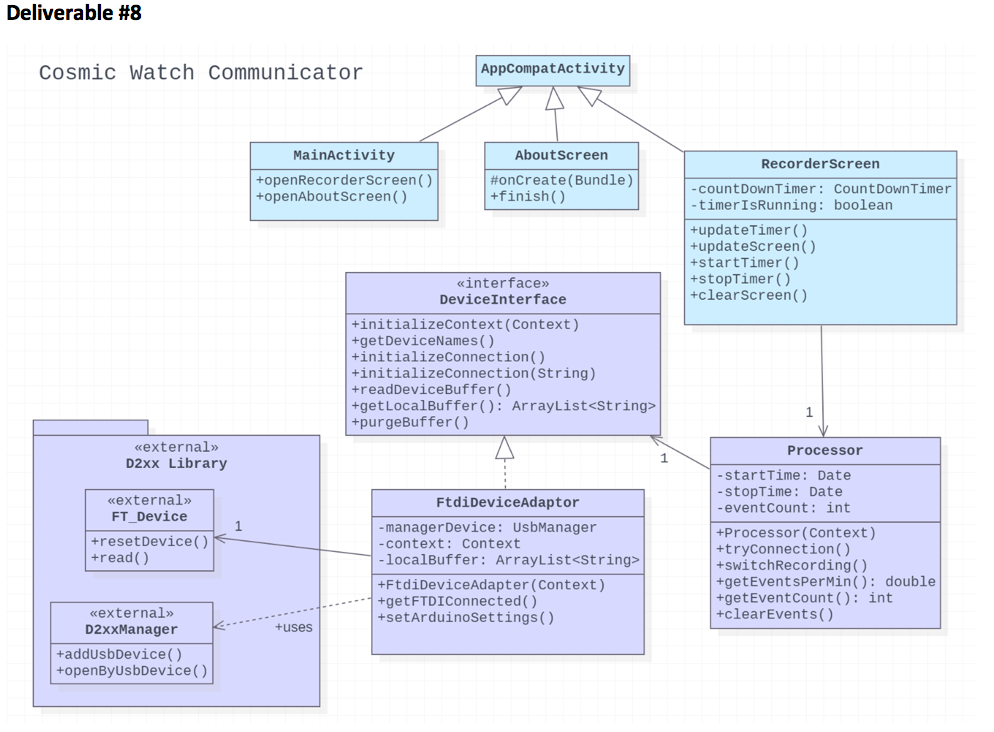
\includegraphics[width=1.2\textwidth]{classdiagramD8.png}
	\caption{A class diagram for our application. Classes that are part of the Adapter design pattern are shown in purple}
\end{figure}


\subsection*{8-2: Explanation}


We decided to implement the Adapter design pattern in our project. In our implementation, the Processor class acts as a client. The target interface is the DeviceInterface class, which contains methods used by the Processor to communicate with the muon detector. The FtdiDeviceAdaptor implements this interface to translate requests from the Processor to the third-party D2xx Library. This library is the adaptee which directly handles connecting to the muon detector.

This pattern was chosen to make our product more flexible in future updates. As our application develops, it may need to support reading data from devices that are not compatible with the external D2xx library. With our updated code, we can now use adapters implementing DeviceInterface to handle specific cases.

With this design pattern, the Processor only uses methods defined by the DeviceInterface to receive data from an external device, regardless of the type of device it is. This reduces coupling since the Processor is only associated with the interface, and not individual adapters. The cohesion of classes has also been increased, since each adapter added will handle a particular type of device, rather than having one class managing many at once.


\section*{Deliverable \#9}

See PowerPoint presentation in the submitted .zip file.


\section*{Deliverable \#10}

After finishing the main functional requirements of our app, we sent the demo video from Assignment 2 to our client, Dr. Jason Donev:

\begin{figure}[h] \centering
	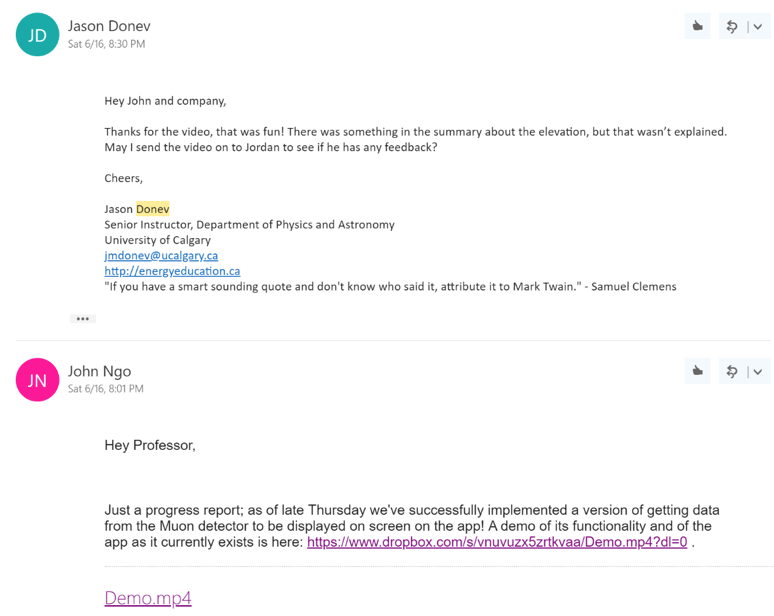
\includegraphics[width=0.9\textwidth]{email1.png}
\end{figure}

\newpage
Jordan was a student of Dr. Donev who created the muon detector that we used to test our app. Thanks to our client, we were luckily able to receive some feedback from him as well.

\begin{figure}[h] \centering
	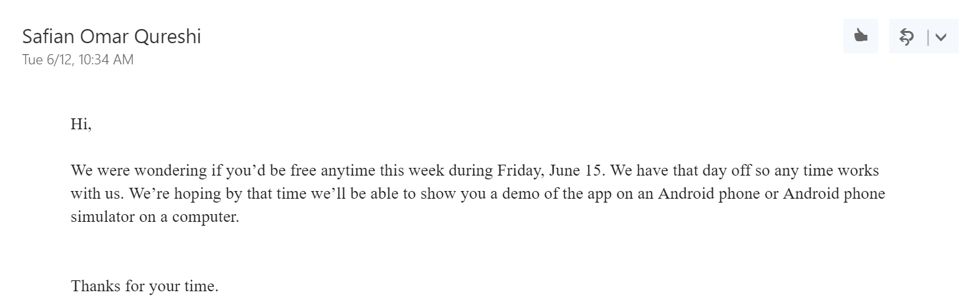
\includegraphics[width=1.08\textwidth]{email2.png}
\end{figure}

We had slight miscommunications when arranging a time to meet Dr. Donev before our class presentation. Thankfully, we found a new time to meet under short notice: 

\begin{figure}[h] \centering
	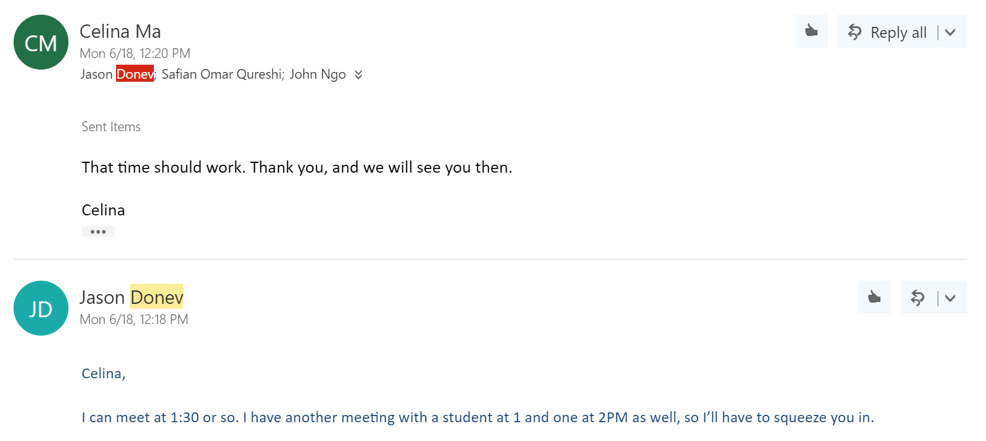
\includegraphics[width=1.08\textwidth]{email3.png}
\end{figure}

Our final meeting with Dr. Donev was on Monday, June 18th. Omar was unable to attend this meeting, but John and Celina were present.


\begin{figure}[h] \centering
	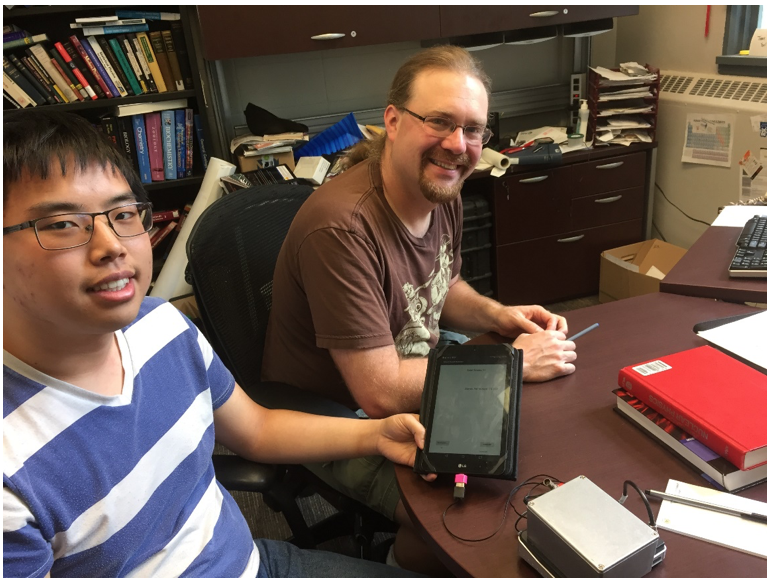
\includegraphics[width=0.9\textwidth]{client1.png}
	\caption{John and Dr. Donev testing out the muon detector app during meeting.}
\end{figure}

As a pleasant surprise, Dr. Donev also introduced us to a visiting nuclear physicist, whom he was speaking with just before our appointment. We briefly explained our application to her and allowed her to try it. It was helpful to see someone unfamiliar with our system interact with it for the first time; she was interested in our app and thought the interface was intuitive.

After the nuclear physicist left, we continued to discuss our app with Dr. Donev. The implementation of our product’s basic functional requirements was complete at this point, so we did not have much to ask about regarding the assignment. We mainly discussed where to take our project in the future. 

Dr. Donev suggested that our app should allow the user to change how long a data recording session lasts, since it only allows the user to record for one minute. We also talked about implementing the data log feature that had been desired since the start of the project. Dr. Donev provided his physics knowledge to estimate how many muon events the app would need to store in extreme conditions, which we wanted to know due to our memory concerns. The meeting ended with Dr. Donev wishing us luck with the project and hoping to hear about our progress in the future.

Overall, Dr. Donev has been a fantastically helpful and supportive client for our team. He was always willing to give suggestions for improvement and meet with us, despite his busy schedule. Again, our greatest challenge with communicating with our customer was finding convenient times to meet in-person. We struggled a bit with rescheduling meetings and beginning appointments on time, but we still made the most of the time we had. For the most part, communication about the project itself was successful, with misunderstandings being resolved quickly.







\end{document}